% \documentclass[twoside,openright]{report}
\documentclass{report}

\usepackage{graphicx}
\graphicspath{{graphics/}}
\usepackage[labelfont=bf]{caption}
\usepackage{placeins}

\let\Oldsection\section
\renewcommand{\section}{\FloatBarrier\Oldsection}
\let\Oldsubsection\subsection
\renewcommand{\subsection}{\FloatBarrier\Oldsubsection}
\let\Oldsubsubsection\subsubsection
\renewcommand{\subsubsection}{\FloatBarrier\Oldsubsubsection}

\usepackage{hyperref}
\usepackage[nottoc,numbib]{tocbibind}

\usepackage{listings}
\usepackage{xcolor}
\definecolor{listinggray}{gray}{0.9}
\definecolor{lbcolor}{rgb}{0.9,0.9,0.9}
\lstset{
backgroundcolor=\color{lbcolor},
    tabsize=4,    
%   rulecolor=,
    language=[GNU]C++,
        basicstyle=\scriptsize,
        upquote=true,
        aboveskip={1.5\baselineskip},
        columns=fixed,
        showstringspaces=false,
        extendedchars=false,
        breaklines=true,
        prebreak = \raisebox{0ex}[0ex][0ex]{\ensuremath{\hookleftarrow}},
        frame=single,
        numbers=left,
        showtabs=false,
        showspaces=false,
        showstringspaces=false,
        identifierstyle=\ttfamily,
        keywordstyle=\color[rgb]{0,0,1},
        commentstyle=\color[rgb]{0.026,0.112,0.095},
        stringstyle=\color[rgb]{0.627,0.126,0.941},
        numberstyle=\color[rgb]{0.205, 0.142, 0.73},
%        \lstdefinestyle{C++}{language=C++,style=numbers}’.
}
\lstset{
    backgroundcolor=\color{lbcolor},
    tabsize=4,
  language=C++,
  captionpos=b,
  tabsize=3,
  frame=lines,
  numbers=left,
  numberstyle=\tiny,
  numbersep=5pt,
  breaklines=true,
  showstringspaces=false,
  basicstyle=\footnotesize,
%  identifierstyle=\color{magenta},
  keywordstyle=\color[rgb]{0,0,1},
  commentstyle=\color[rgb]{0,0.5,0},
  stringstyle=\color{red}
  }

\usepackage{filecontents}

\usepackage{setspace} 

\newcommand{\specialcell}[2][c]{%
  \begin{tabular}[#1]{@{}c@{}}#2\end{tabular}}



\begin{document}

\begin{titlepage}
    \begin{center}
        \vspace*{3cm}
        
        \Huge
        Design And Analysis Of A Plastic Parallel Programming System
        
        \vspace{1.5cm}
        
        \large
        \textbf{Mark Jenkins}
        
        \vspace{2.5cm}

        
\includegraphics[width=0.3\textwidth]{university}

        \vspace{2.5cm}
        
        \textbf{MInf Project (Part 1) Report}\\
        Master of Informatics\\
        School of Informatics\\
        University of Edinburgh\\
        2017
    \end{center}
\end{titlepage}

\setlength\parskip{1em}
\setlength\parindent{0pt}



\begin{singlespacing}

%!TEX root = Report.tex
\begin{abstract}

\setlength{\parskip}{1em}

\noindent Throughout the history of computing, computer programmers and hardware engineers have exploited parallelism, with software and architectural innovation complementing technological improvements to provide increased performance. Architects have exploited bit and instruction parallelism, and now programmers are increasingly exploiting task/data parallelism in their applications.

\noindent Utilizing hardware efficiently is a major research challenge, especially considering that, today, a single program or library needs to deal with multiple different incarnations of the task it is trying to run. These arise from different circumstances, ranging from the hardware it is running on to the task size. Creating a ``one size fits all'' solution has become increasingly difficult, especially for high performance parallel applications. As such, there are solutions to help mitigate this problem (cite petabricks), which utilize this idea of plastic programming, that is, changing the specifics of an implementation depending on the circumstances. However, such solutions are only "plastic" at compile time, and during runtime if circumstances change they cannot adapt. In particular, the most common situation a program may encounter would be the sharing of the computer's resources with other programs. This is again exacerbated for high performance parallel programs, as they typically attempt to use all the resources they can get their virtual hands on.

\noindent It is known that in such a situation with two programs, with careful selection of program parameters, we can obtain a better average runtime for both programs (cite lira paper).

\noindent This paper investigates if we can combine these ideas to create a parallel programming skeleton library where incarnations of its patterns will explicitly work together in this manner, and whether we can obtain any significant difference in performance. We then go on to discuss the ramifications, and how this could be taken further, and possibly used to implement a useful tool for programmers.

\end{abstract}

\tableofcontents

\newpage

\chapter{Introduction}
\label{chapter:introduction}
%!TEX root = ../Report.tex

Throughout the history of computing, computer programmers and hardware engineers have exploited parallelism, with software and architectural innovation complementing technological improvements to provide increased performance. Architects have exploited bit and instruction parallelism, and now programmers are increasingly exploiting task/data parallelism in their applications.

It is recognised that writing correct and efficient parallel programs is hard, (cite \url{http://www.futurechips.org/tips-for-power-coders/parallel-programming.html} or \url{https://parallel.illinois.edu/blog/three-challenges-parallel-programming} or something, \url{https://dl.acm.org/citation.cfm?id=2093943&dl=ACM&coll=DL&CFID=720336161&CFTOKEN=82786616}) as the introduction of parallelism introduces a whole host of new problems, (e.g. unreproducible bugs due to race conditions, and difficult debugging as high level instructions need ot be decomposed  into atomic assembly code to understand what is going on). The sole purpose of multi-threading is improved performance, however parallel programs can often be slower then their serial counterparts, be it due to dependencies or hardware contention. Overhead must be balanced such that we don't introduce so much more work organizing threads and computations that our performance gains disappear.

Utilizing hardware efficiently is a major research challenge, especially considering that, today, a single program or library needs to deal with multiple different incarnations of the task it is trying to run. These arise from different circumstances, ranging from the hardware it is running on to the task size. Creating a ``one size fits all'' solution has become increasingly difficult, especially for high performance parallel applications. As such, there are solutions to help mitigate this problem (cite petabricks), which utilize this idea of plastic programming, that is, changing the specifics of an implementation depending on the circumstances. However, such solutions are only "plastic" at compile time, and during runtime if circumstances change they cannot adapt. In particular, the most common situation a program may encounter would be the sharing of the computer's resources with other programs. This is again exacerbated for high performance parallel programs, as they typically attempt to use all the resources they can get their virtual hands on.

Even when we have an ideal parallel program, often resources are shared between multiple programs and users, leading to resource contention. This is the case for most use cases, from the serious computing resources in data centres, to the low powered hardware of mobile phones. Even in our own computing labs, we have messages to the effect of "Do not leave applications running on this machine" or "please nice your programs", which are often unseen or disregarded.

It is known that in such a situation with two programs, with careful selection of program parameters, we can obtain a better average runtime for both programs (cite lira paper).

The aim of this project is to simplify the challenges of parallel programming and to provide improved performance by utilizing three key ideas:

\begin{itemize}
	\item Co-Scheduling
	\item Plastic Programming
	\item Skeleton Programming
\end{itemize}

and to investigate the performance ramifications. Combining these ideas results in these problems becoming particularly tricky, with many different challenges involved in incorporating them.

The layout of the report is as follows; In \autoref{chapter:background} we will provide an exploration of the ideas behind the report, and give a quick overview of how they are combined. In \autoref{chapter:design}, we will detail the thought process behind the design of our system, and then in \autoref{chapter:implementation} we will then go into the specifics of the implementation of the system. \autoref{chapter:experimental_methodology_and_program} presents a carefully selected series of experiments to assess this system, and in \autoref{chapter:results} we discuss the results of these experiments and their ramifications. \autoref{chapter:future_work} provides a layout the roadmap of future work for the second part of this two year MInf project and beyond. We then end with providing our final thoughts on the topic in \autoref{chapter:conclusion}.

\chapter{Background}
\label{chapter:background}
%!TEX root = ../Report.tex

In this chapter, we will detail the current approaches to parallel programming. We will then explore the three key ideas requisite to this project, such that we can discuss how they are combined and the implications.

The main new idea in this project is that of dynamic contention aware scheduling and optimization. It has been shown to be an important factor in multiprogramming systems with performance implications \cite{lira}. Plasticity is a technique to respond to this challenge, and take it further. This results in complex code, making it hard to ensure correctness. So we use skeletons to abstract this complexity away from the programmer. It also has the nice side effect of dividing the challenge into a pattern-by-pattern basis.

In this project we will produce such skeletons, and investigate the performance implications of these ideas, in order to evaluate whether they will have a significant effect.



\section{Current Solutions}

Current solutions for parallel programming include:

\begin{itemize}
	\item Pthreads (POSIX Threads)
	\item MPI 	   (Message Passing Interface)
	\item OpenMP   (Open Multi-Processing)
\end{itemize}

These are the more conventional methods of parallel programming.

Pthreads provides the highest level of fine grain control, leaving most of the work to the programmer. As such, some parallel processing techniques may only be possible with Pthreads. It is implemented in the POSIX library, and is well integrated with the standard GNU compiler collection (\textbf{gcc}). Pthreads only makes sense with shared memory architectures.

MPI is a communication library, and as such mostly details how processes can communicate. It is the dominant model used in the high performance computing industry today \cite{mpi}. It can not only be used for a parallel program running on a single machine, but can also be used to implement a parallel program running on a distributed memory system.

OpenMP is comprised of compiler directives, runtime library routines, and environment variables. It is mostly used for loop parallelization, and is much higher level. It is also not limited to C. Like Pthreads, OpenMP is intended for shared memory architecture as it is thread bound.

Each of these methods have their own way of dealing with the complications introduced with parallel programming, which range from race conditions to limited scalability. These new problems can certainly be overwhelming to a traditionally sequential application programmer, so much so that there are entire books dedicated to the use of each of these particular parallel programming methods. 



\section{What Is Contention Aware Scheduling?}

It is known that in multiprogramming systems, with many programs running simultaneously, the choice of program to socket mapping significantly affects the performance of the system \cite{lira}. Just considering two programs running on the same socket, we can see from the graph in figure \ref{fig:lira_pairwise_speedup} that certain programs perform differently with others, with some strange cases where the programs actually display better performance when running in contention with another. This problem is called co-scheduling.

So with this evidence, we can see that if we take into account such factors in our scheduler, we may obtain better overall performance. The outcome of the LIRA paper concludes that throughput gains of 3-7\% can be seen. Socket/resource aware scheduling in this manner is called a contention aware scheduler. Adding in the plastic programming idea could make this particularly powerful, because we know and control the specifics of the implementations, and not only can we control what program runs where, we can also adjust the implementation the program is using.

\begin{figure}
	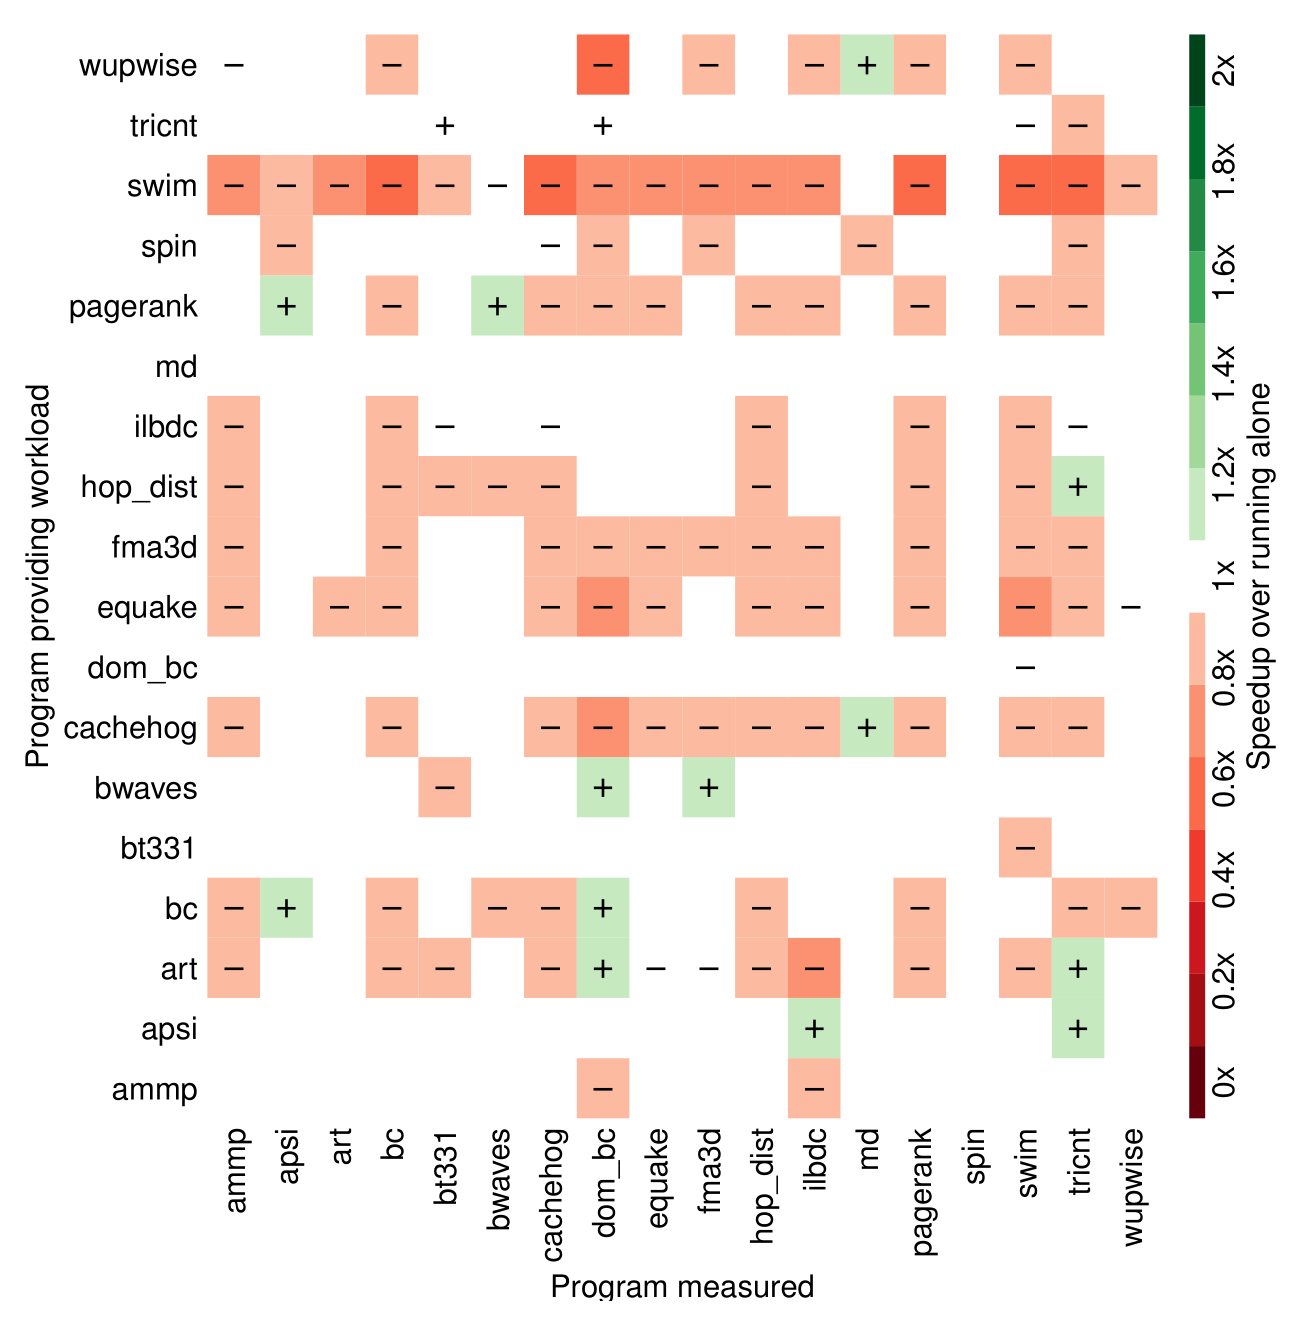
\includegraphics[width=\textwidth]{graphics/lira_pairwise_speedup.png}
	\caption{Taken from the LIRA paper \cite{lira}: Pair-wise speedup of programs, comparing sharing a socket to using separate sockets. Boxes annotated with a $-$ indicate cases where performance decreased, and $+$ where performance increased. In LIRA, this information was used to select which programs, from a given workset, should be scheduled concurrently, in order to maximize performance.}
	\label{fig:lira_pairwise_speedup}
\end{figure}



\section{What Is Plastic Programming?}

When programming an algorithm, there are often many choices about the specific implementation which can greatly affect performance, and the best choice depends on the circumstances of the problem. We tend to have more choices with parallel programs, but this is the case even for sequential programs. As an example, for a sorting problem with a large input size, radix sort would perform best, whereas for a small input size, insertion sort would be better. So naturally, in the interests of performance, we can conceive of a better overall implementation by combining the two approaches, so if the task size is large we would use radix sort, and then once it is reduced (for example, in a recursive algorithm,) we would use insertion sort. 

An example of such a hypotheticaL situation can be seen in figure \ref{fig:plastic_graph}, which shows three algorithms with different runtime curves, which depend upon the array size. Combining these algorithms would provide an improved algorithm, with D1 and D2 showing the optimal decision points where a plastic programming system should switch algorithms.

Such compositions are commonplace, such as the sorting example discussed in the PetaBricks paper introduction \cite{petabricks}. Compared to PetaBricks, our implementation of plastic programming will be a little different. With the PetaBricks system, the programmer must specify multiple implementations for the compiler to switch between. In our system, we provide the various implementations in our library, meaning no extra effort is required from the programmer.



\begin{figure}
	\centering
	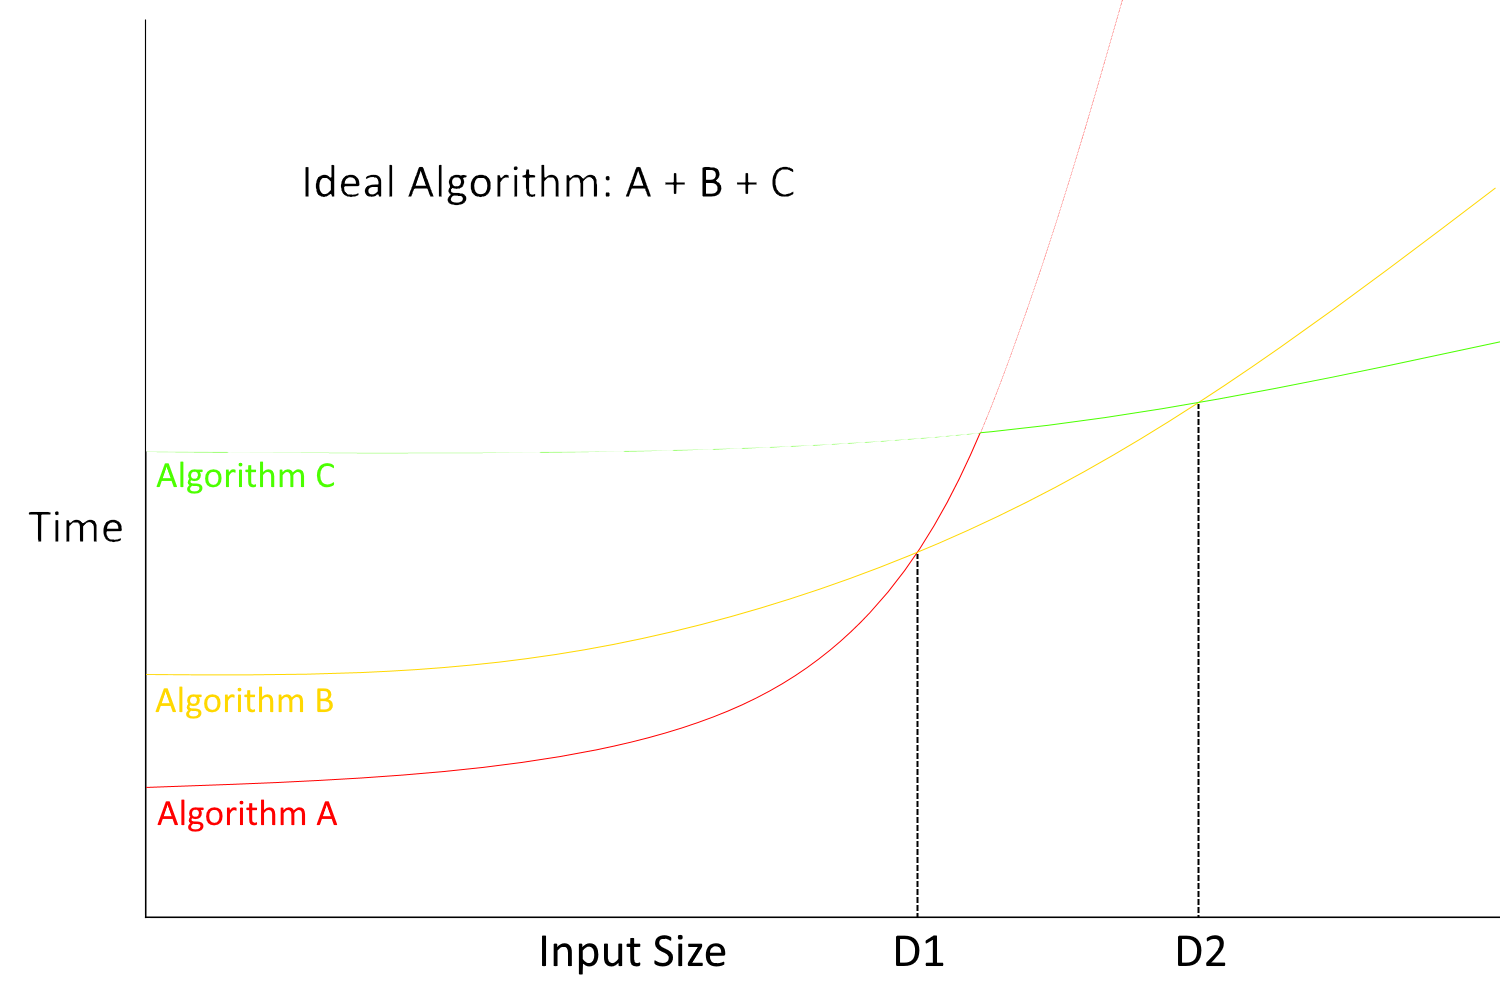
\includegraphics[width=\textwidth]{plastic_graph}
	\caption{A graph showing three algorithms with different runtime curves, which depend upon the array size. Combining these algorithms would provide an improved algorithm, with D1 and D2 showing the optimal decision points where a plastic programming system should switch algorithms}
	\label{fig:plastic_graph}
\end{figure}



\section{What Is Skeleton Programming?}
\label{section:background_what_is_skeleton_programming}

Skeleton programming is a high-level programming model. Skeletons allow us to abstract away all the complexity involved in parallel programming, plastic programming, and co-scheduling. The essence of skeleton programming is that the skeleton provides the core structure of an algorithm, the user provides some code (In our case, a function), which then produces a correct program for the task at hand. The skeleton handles the hard-work of providing and optimizing the code (In our case, dealing with parallelism, plasticity, and co-scheduling). 

The consequences of this are twofold:

\begin{itemize}
	\item Errors are reduced substantially, as parallel programming is not easy, even without plasticity and contention aware scheduling.
	\item We can assess the program's complexity, since we know the algorithmic details of the skeleton.
\end{itemize}

Typically, multiple skeletons are combined to produce a more complex program, for example, a common combination is map and reduce (specific skeletons will be discussed in section \ref{section:design_skeleton_foundation}.) The ability to combine skeletons makes them a powerful tool, allowing programmers to easily create clean complex programs.

Previous work to make parallel programming simple utilizing skeletons includes:

\begin{itemize}
	\item SkePU \cite{skepu}
	\item The Münster Skeleton Library Muesli
\end{itemize}

These methods simplify the problem, with both utilizing skeleton programming to do so. Since each SkePU skeleton has multiple implementations, and SkePU automatically selects the expected fastest implementation variant, it is the closest to the system we wish to implement. In contrast to our system, this selection is not dynamic, i.e. it does not change during runtime. 



\section{Summary}

In this chapter, we described the three fundamental concepts behind this project, contention aware scheduling, plastic programming, and skeleton programming. With just contention aware scheduling, we can achieve greater performance \cite{lira}. In this project we will take this idea further, adding plastic programming, so we can adapt the implementation of programs at runtime. This lets us change the implementations to ones which we know work well together. Combining these two ideas results in considerable complexity, so to make it simple for a programmer to use and easier for us to program, we use skeletons to abstract this complexity. The details of this complexity and how these ideas are combined are described in chapter \ref{chapter:implementation}.

The intent of this project is to explore the extent to which this approach can outperform a contention aware scheduled system which doesn't utilize plasticity. This is the plan for the first year of this Minf project, with the structure of the second year detailed in chapter \ref{chapter:future_work}.

\chapter{Design}
\label{chapter:design}
%!TEX root = ../Report.tex

In this chapter, we will discuss the design of the system created to investigate the problem in hand, and detail how such a system could be extended for the future.



\section{System description}

The ideas described in the background section are combined to produce a skeleton programming library which utilizes plasticity and contention aware scheduling. To keep it simple, we build the system incrementally, starting with a single parallel pattern, later adding plasticity and contention aware scheduling. 



\subsection{Skeleton Foundation}
\label{section:design_skeleton_foundation}

As discussed in the background section, one of the key ideas behind the project is that of skeleton programming, using predefined patterns to aid the programmer. Possibly the most common skeleton is map, which is a skeleton that takes a function, an array of data, and applies the function to each member of the array. The map operation itself is inherently parallelizable, since each `task' (processing one element of the input array) is independent, so we can simply assign different chunks of the input array to different threads. This is called an ``embarrassingly parallel'' problem. 

Other such patterns include map-array, reduce, and scan. These are all implemented in SkePU with a corresponding skeleton (as described in section \ref{section:background_what_is_skeleton_programming}.) In our case, we will focus on the map-array pattern, with further patterns left for possible future work. Map-array is similar to the map pattern in that it applies a given user function to each element in a list, however map-array also allows the function to access a user provided array. A diagram to better explain this is given in figure \ref{fig:skepu_skeletons}.

Map-array was chosen as the focus of the project as the map pattern is likely the most well known pattern and certainly one of the most useful, and map-array provides further functionality on top of this. It also provides a good basis for developing further patterns, and allows for the testing of more complex situations, which will be covered in chapters \ref{chapter:experimental_methodology_and_program} and \ref{chapter:future_work_and_conclusions} of this report.



\begin{figure}
	\centering
	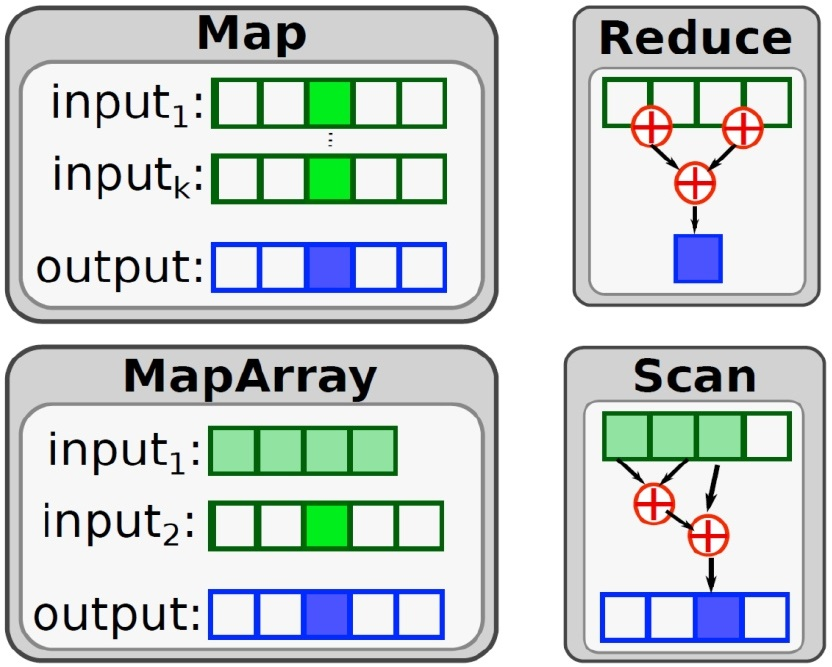
\includegraphics[width=0.7\textwidth]{graphics/skepu_skeletons.jpg}
	\caption{Taken from SkePU documentation: Examples of patterns}
	\label{fig:skepu_skeletons}
\end{figure}



\subsection{Adding Plasticity}
\label{subsection:design_adding_plasticity}

To implement plasticity, we add the ability to vary three key aspects of the implementation of a single instance of the map-array skeleton:

\begin{itemize}
	\item Thread count - The number of threads we split the tasks between
	\item Thread pinnings - The particular CPU core each thread runs on
	\item Schedule - How to divide tasks between threads
\end{itemize}

The thread count and pinnings are self explanatory. The schedule however requires some explanation.

The most basic method to divide the tasks is to give an equal amount to each thread. This is fine if the complexity of the tasks is uniform, but if it is biased (e.g. tasks in the first portion of the array are more complex than the rest), the amount of computation to be done by each thread is imbalanced. This is because we have idle cores during computation, since the threads with more work will still be computing once the others have finished. This downtime is a wasted resource in a multi-threaded execution. However, if we allocate the tasks differently, we can obtain better performance, as illustrated in figure \ref{fig:schedule_optimization}, where the improved schedule runs twice as fast as the simple one.

So load balancing a workload is critical to performance in such a multi-threaded application. However, optimizing the task distribution in this manner is a non-trivial problem, and it depends upon the computation to be done as well as the number of threads and other resources available at runtime.

A solution to this problem is to provide many different task distributions, and let the user pick or the machine select which distribution to use. OpenMP documentation calls these schedules, and some examples of these are:

\begin{itemize}
	\item Static - An equal number of tasks allocated to all threads
	\item Dynamic individual - Each thread retrieves one task at a time, and once completed, it goes back for more
	\item Dynamic chunks - Each thread retrieves N tasks at a time, and once completed, it goes back for more
	\item Tapered - Each thread starts by retrieving N tasks at a time, and as the computation continues, it retrieves fewer and fewer
\end{itemize}

Thread count and schedule were chosen as they seem the most critical to performance, and thread pinnings was added as this is was investigated in the LIRA paper \cite{lira} as a factor contention aware scheduling could exploit.

Once we have added plasticity, we can experiment with the specifics of an implementation, and see how they affect the performance of the system. This would be the use case of utilizing our library with no other program running, (i.e. no contention aware scheduling), and we can explore how we can adapt the program using plasticity at runtime in this case. We may be able to improve performance even under these conditions, depending upon the configuration of the machine (e.g., are there more CPU cores available) and the problem (e.g. do we have many small tasks or few large tasks.) 



\begin{figure}[!]
	\centering
	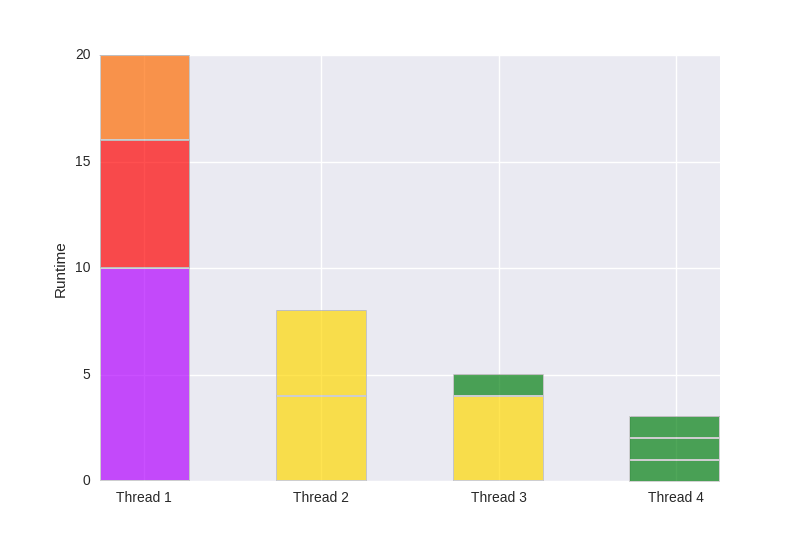
\includegraphics[width=0.9\textwidth]{graphics/unoptimized_schedule.png}
	\caption{A worst case scenario of a static schedule assigning each thread an equal number of tasks. Suppose we have a set of twelve independent tasks with the following set of execution times (These would be unknown to the scheduler): \{10, 6, 4, 4, 2, 2, 2, 2, 1, 1, 1, 1\}. With four threads, a simple division of tasks would be three tasks each distributed in order. This figure illustrates this distribution of work. Note that the total execution time is 20 time units.}
	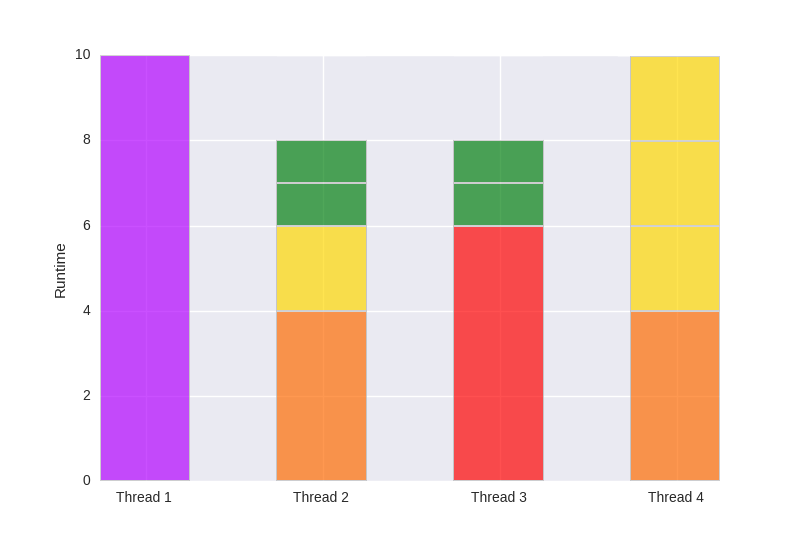
\includegraphics[width=0.9\textwidth]{graphics/optimized_schedule.png}
	\caption{An optimized version of the previous schedule. Here we have the same set of tasks, but we have a better distribution of work, so the total execution time is 10 time units.}
	\label{fig:schedule_optimization}
\end{figure}



\subsection{Contention Aware Scheduling}
\label{subsection:design_contention_aware_scheduling}

To add contention aware scheduling, we need multiple applications using our library to be able to collaborate, and adapt their behaviour accordingly. To do this, we use a separate controller application, with which all instances of our program can communicate. This provides a single known point of contact, and a designated thread for computing program parameters with respect to all aspects of the system.

Once our programs can communicate, and we can control each aspect of them, we can implement contention aware scheduling. In this phase of the project, we simply program a set of predefined actions for the controller to take, in order to manually control what each implementation does, as we are only investigating if this approach seems promising. We leave implementing some algorithm for automatic parameter tuning for future work.

A diagram showing the high level communication model is given in figure \ref{fig:communication_structure}. This is expanded upon in section \ref{section:implementation_contention_aware_scheduling}, showing specifics about the implementation.

With contention aware scheduling, we can experiment with multiple programs running on a system at once. An example of how contention aware scheduling can be enhanced with plastic programming is given in figure \ref{fig:plastic_contention_aware_scheduling}.



\begin{figure}
	\centering
	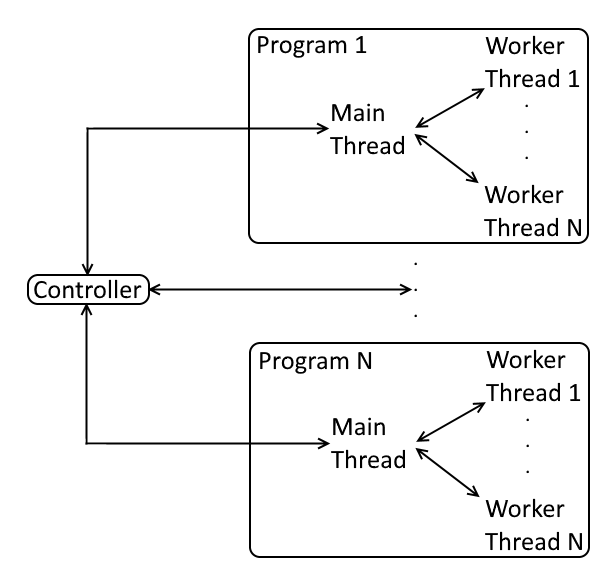
\includegraphics[width=\textwidth]{graphics/communication_structure.png}
	\caption{High level communication model of the system, with an arbitrary number of programs, with an arbitrary number of threads. Two way communication occurs between the controller and each main thread, and then between each main thread and its worker threads.}
	\label{fig:communication_structure}
\end{figure}

\begin{figure}
	\centering
	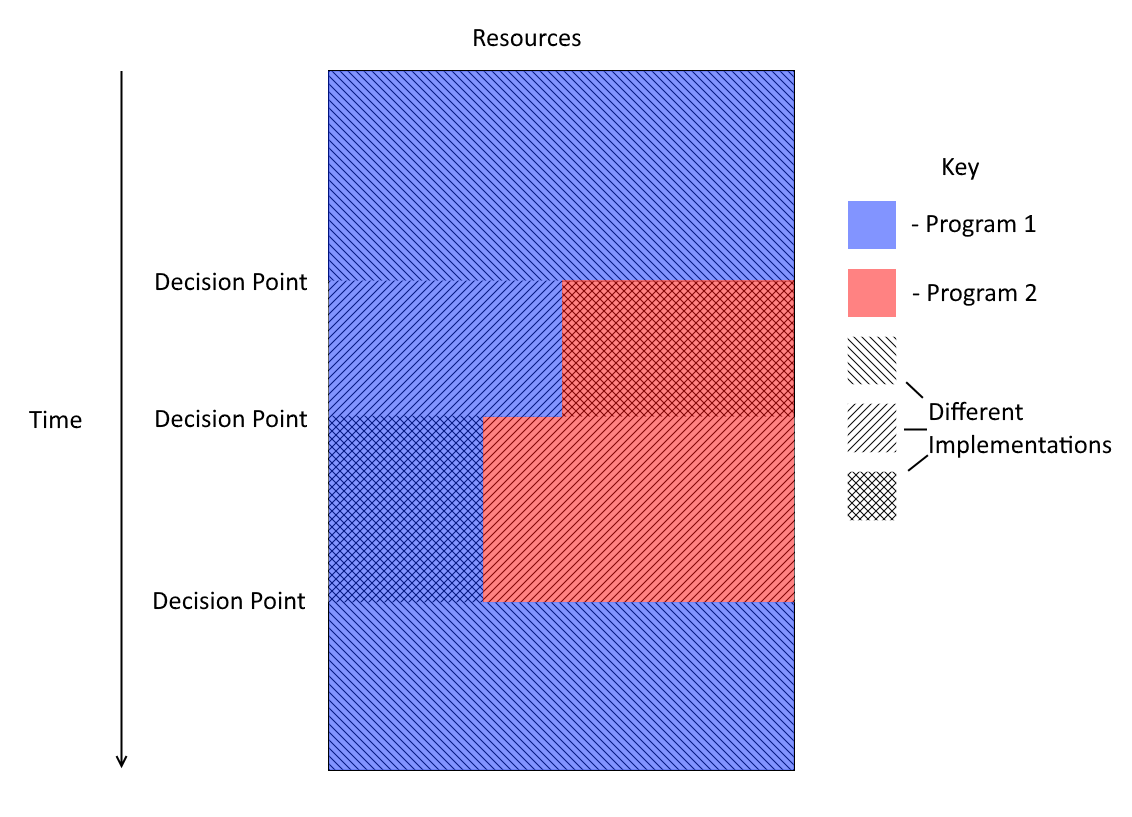
\includegraphics[width=\textwidth]{graphics/plastic_contention_aware_scheduling.png}
	\caption{An example of how contention aware scheduling can be enhanced with plastic programming. We have two programs, represented by different colours. As time progresses, we see that when program 2 launches, we have a decision point. Here, the system decides how many resources to give each program and what implementation they should use, according to what is optimal (in this project, we do this manually.) \\ \\ Moving further in time, we have another decision point. This one is triggered by some other change in the machine, which means the optimal configuration has changed. So the system updates the configuration of each program, and continues. \\ \\ Program 2 then terminates, triggering another decision point, and the system again updates the configuration.}
	\label{fig:plastic_contention_aware_scheduling}
\end{figure}



\subsection{Evaluation}

To properly evaluate the outcome of this project, we need some way of testing the libraries performance. To this end, we implemented a synthetic program which calls the skeleton with an artificial workload, collecting and recording metrics detailing the libraries performance with different parameters.  

We also need points of comparison in terms of performance. So, in addition to our synthetic program, we also implement an equivalent sequential and an OpenMP version, in which we can vary similar parameters and produce comparable statistics. 

The detailed experimental program will be discussed in chapter \ref{chapter:experimental_methodology_and_program}.

\chapter{Implementation}
\label{chapter:implementation}
%!TEX root = ../Report.tex

In this chapter, we present specific implementation details of the project, and cover the problems that occurred and how they were solved.

We start with the implementation of a basic skeleton, then  we cover adding plasticity, and contention aware scheduling. Finally, we finish by covering the applications developed to evaluate the project.

C++ was chosen as a basis, since it's fast, and provides language constructs such as templates and overloading. Another, personal, reason is that I wished to learn something new, as I had not used C++ before. 

The parallel backend that the system is based upon is Pthreads due to its wide availability, and the level of fine control. It allows us to tune all parameters of the program and implement functions which are not possible with other solutions, e.g. detailed metric analysis. 



\section{Skeleton Foundation}
\label{section:implementation_skeleton_foundation}

The first skeleton we will implement is the map-array skeleton, as described in section \ref{section:design_skeleton_foundation}. It is reasonably straight forward to create a sequential skeleton, using c++ templates to create a templated function which takes a function amongst other things as it's arguments. This will be our skeleton. The interface of our skeleton is given in figure \ref{fig:map_array_interface}, and a usage example in figure \ref{fig:map_array_usage_example}.



\begin{figure}
	\begin{lstlisting}

	template <typename in1, typename in2, typename out>
	void map_array(deque<in1>& input1, 
				   	deque<in2>& input2, 
				   	out (*user_function) (in1, deque<in2>), 
				   	deque<out>& output, 
				   	string output_filename = "", 
				   	parameters params = parameters())

	\end{lstlisting}

	\caption{Interface of our map\_array skeleton. The first four variables are the two input arrays, the function to apply, and the output array respectively. The output\_filename variable is the filename to record the metrics output in, and params sets up the initial parameters we will use. These last two are optional.}
	\label{fig:map_array_interface}
\end{figure}



\begin{figure}
	\begin{lstlisting}

	int user_function(int in1, deque<int> in2) {
		return in1 + in2[in1];
	}

	int main() {
		// Inputs.
		deque<int> input1(ARRAY_SIZE);
		deque<int> input2(ARRAY_SIZE_2);

		/*
		 * Put data in inputs.
		 */

		// Output.
		deque<int> output(ARRAY_SIZE);

		// Start mapArray.
		map_array(input1, input2, user_function, output);

		/*
		 * Record output.
		 */
	}

	\end{lstlisting}

	\caption{A usage example of map\_array, here we apply our user\_function to each element of input1. The size of our two input arrays need not match, but the size of the input1 and output arrays must.}
	\label{fig:map_array_usage_example}
\end{figure}



\begin{minipage}{\textwidth}

Parallelizing this presents two problems, namely:

\begin{itemize}
	\item How to divide tasks amongst threads (In map array, one task is one application of the user function to an element of the input array)
	\item How many threads should be used
\end{itemize}

\end{minipage}
 
In a basic skeleton, both of these parameters must be specified beforehand and will not change at runtime. The ability to vary them would provide the different implementations necessary for the plasticity portion of this project.

To implement multiple schedules, we use a bag of tasks object. A bag of tasks is a collection of independent, usually similar tasks which are to be executed. It is a model which is usually combined with some form of parallelism.

Each thread will be given the location of the same bag, and will retrieve a specified number of tasks at a time from the bag. Since each schedule essentially consists of retrieving a different number tasks, we can use this to implement the basic schedules (Static, Dynamic chunks, Dynamic Individual). More complex schedules can easily be added in the future, as they can reuse the get tasks method, an simply adjust how many tasks each thread retrieves at one time.

The bag also provides the main source of inter-thread communication using shared memory, and contains various semaphores for controlling the threads. This will be expanded upon in sections \ref{section:implementation_adding_plasticity} and \ref{section:implementation_contention_aware_scheduling}.

This bag of tasks object also gives us the basis for further extensions, such as using multiple bags, adding task stealing, or adding tasks to the bag during computation.

Providing a variable number of worker threads is simple now that we have the bag of tasks, all we need to do is to adjust our initial calculations when calculating how many tasks each thread should receive according to the schedule. These worker threads will be spawned by the original thread, the ``main'' thread. It will block until all computation is complete, it will then join with each of the worker threads.



\section{Adding Plasticity}
\label{section:implementation_adding_plasticity}

We already have a sort of compile time plasticity in our system, in that we can choose some parameters of the skeleton before compilation. We can choose the number of worker threads and the schedule used. The other main aspect we would like to control is what CPU core each thread executes on. This is called processor affinity or thread pinning. This was added to the skeleton by adding control variables to the bag of tasks, which control the CPU affinity of each thread. Each thread then simply sets it's affinity to the intended CPU.

To add runtime plasticity, we need to be able to change the implementation of the skeleton on the fly. The most straightforward method of achieving this is to stop all computation, terminate worker threads, update the parameters, and resume computation. In a basic skeleton, (as described at the end of section \ref{section:implementation_skeleton_foundation},) the main thread would block until the computation is complete, and then would join with each of the worker threads. We change this so that, instead of blocking, it monitors the computation and can instruct the threads to terminate at any point (using the afore mentioned bag of tasks described in section \ref{section:implementation_skeleton_foundation} for communication). This allows it to prematurely terminate the computation, and then restart it with the new desired parameters. 

When this switching is done and what the new parameters should be is another matter. A future system would calculate these things dependent upon the current state of the system, but for our preliminary investigation, we manually produce them in a synthetic environment, and communicate them to the main thread using the controller application, as described in section \ref{section:implementation_contention_aware_scheduling}.

An obvious optimization of this system would be to modify the implementation without the need to terminate threads. This graceful switching of the implementation is left for future work, as this optimization is very complex, and would likely result in a marginal speedup proportional to the number of times we wish to change the implementation. We don't plan on switching implementations excessively, and any delay added could be overcome in testing by increasing the input size, and this project is only investigating if this approach to parallel programming is promising.

Another optimization would involve modifying the static schedule. In our implementation, worker threads only check if they should terminate when they contact the bag for more tasks. Since the static schedule means they only contact the bag at the start of the computation, once they have started, they cannot be interrupted. To optimize this, and make a "plastic" static schedule, we could change the communication method so that worker threads can be interrupted. This hasn't been necessary for our current work, and as such has been left for future work.



\section{Contention Aware Scheduling}
\label{section:implementation_contention_aware_scheduling}

As detailed in section \ref{subsection:design_contention_aware_scheduling} of the design chapter, we will use a separate controller application to co-ordinate and control all programs using our library. This simplifies the implementation significantly, as it gives us a single point of contact, and a single place to calculate an optimal configuration for each program. To achieve this, we need our separate controller application, and two main additions to our system:

\begin{itemize}
	\item Inter-process communication
	\item Separate communication/control thread for each program
\end{itemize}

We use the zeromq library to provide inter-process communication for it's speed, although it could be replaced with another method. It uses tcp sockets, and serves to simplify inter-process communication. Currently I have made simple use of zeromq for now, and may optimize it in the future. For inter-thread communication (between a main thread and worker threads), we use shared memory, again for speed and simplicity.

In order to communicate with the controller while a program is using our library, we utilize our main thread, which will manage the worker threads, switch implementations when instructed, and will clean up after we have finished our computation. The main thread communicates with the controller, registering with it when we start and de-registering once complete. During computation, it listens to messages from the controller using non-blocking communication. This allows us to also check if we are finished processing. For the initial registration and de-registration, we use blocking communication, as these messages are vital to the system. This system is illustrated in figure \ref{fig:controller_flowchart}, which expands upon figure \ref{fig:communication_structure}, showing implementation details.



\begin{figure}
	\centering
	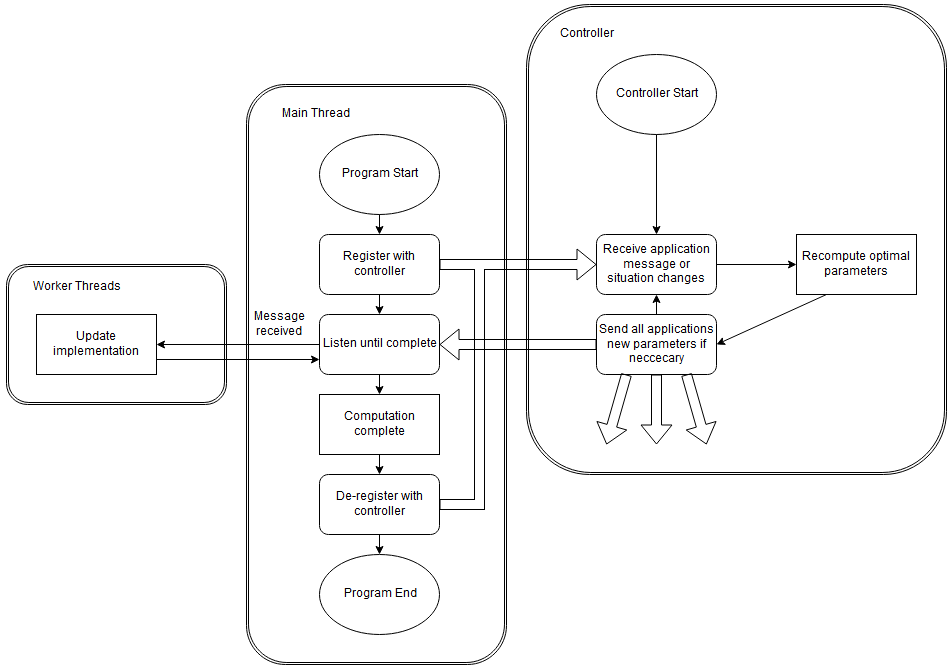
\includegraphics[width=\textwidth]{graphics/controller_communication_flowchart.png}
	\caption{Communication model for communications between applications and the controller. Thin lines represent program flow, thick lines represent inter-process messages.}
	\label{fig:controller_flowchart}
\end{figure}



\section{Testing Programs}

To evaluate our library, we need programs to run and test the library under differing conditions, and we need programs to represent competing approaches to parallel programming. 

The main map-array test application is a tool which can read experiment parameters from a configuration file, and then run each experiment in sequence, recording various metrics for later analysis. This provides a convenient framework for carrying out experiments, and easily enables us to queue up a set of experiments. This is important because such experiments can take hours.

For meaningful analysis, we need to synthesize a workload. One which we can scale, so we can test different sized tasks and varying task distributions. To do this we use the Collatz function to generate a CPU intensive workload. A constant starting number is used, and the sequence is repeated multiple times, to scale the workload.

The comparison programs consist of a purely sequential implementation, and an OpenMP implementation. These were chosen because the former represents an implementation a traditional sequential programmer would use, and OpenMP because it is a popular method of parallelizing code, with a focus on performance and a simple interface. They are set up such that they can use the same synthetic workload we use for testing our library.

The final tool we constructed for evaluation is a python program which was used to create graphs from the generated data.

\chapter{Experimental Methodology And Program}
\label{chapter:experimental_methodology_and_program}
%!TEX root = ../Report.tex

\newif\iflabela
\newif\iflabelb
\newif\iflabelc
\newif\iflabeld
\newif\iflabele



The primary goal of this project is to investigate if we can achieve better performance using the combination of plasticity and contention aware scheduling. Accordingly, we will focus our experiments on evaluating the performance of the system. To this end, we have created a carefully designed set of experiments to assess the system under different conditions, conditions which may be found in future applications. In this chapter we describe our evaluation methodology and the particular experiments we will run. The outcome of each experiment will be discussed in the results chapter in the same order they are presented here.



\section{Evaluation Methodology}

All experiments were run on an Ubuntu virtual machine, with four cores at 4GHz, 4096MB of memory, and the rest of the system at idle. All programs were compiled at optimization level 3, and every result averaged over 50 repeats.

Multiple different statistics can be collected for each thread:

\begin{enumerate}
	\item Total runtime
	\item Time spent doing work
	\item Time spent in overhead
	\item Time blocked by main thread
	\item Number of tasks completed
\end{enumerate}

In these experiments however, we will focus on total runtime, as we are mostly concerned with the overall performance. The other statistics were mostly used during development. Experiment 1 investigates the impact of the collection of these detailed metrics.



\section{Programme of Experiments}

In this section we detail each experiment, the thought process behind it, how it will be executed, and the expected results if appropriate. The actual results will be presented in chapter \ref{chapter:results}, where we will compare them with our expectations and discuss their implications.

In each experiment we will vary a different set of parameters. These parameters can be partitioned into three separate classes; application input parameters, resources granted, and skeleton parameters. More parameters can be added, (e.g. different resources granted,) but this is left for future work, as currently we only want a preliminary investigation into these ideas. The set of parameters are:

Application Input Parameters:

\begin{itemize}
	\item Number of tasks - The number of tasks to be carried out
	\item Task grain - The complexity of the tasks, measured in the number of repeats of the Collatz function.
	\item Task grain distribution - If we have range of task grains, this describes how they distributed throughout the input array. Possible values are uniform (evenly distributed throughout,) and biased (The more complex tasks are gathered together in the first 1/N portion of the array, where N is the number of threads. This is the worst case scenario for the static schedule.)
\end{itemize}

Resources Granted:

\begin{itemize}
	\item Number of CPU cores - The amount of CPU cores provided in the machine.
\end{itemize}

Skeleton Parameters:

\begin{itemize}
	\item Number of threads used - The number of threads our program uses for multi-threading.
	\item Thread pinning - The configuration of threads pinned to CPU cores. They are either uniformly spread across all CPU cores, or left unpinned (we call this situation ``anarchy''.)
	\item Schedule - How the tasks are distributed amongst threads. See section \ref{subsection:design_adding_plasticity} for the possible schedules.
\end{itemize}

Our first experiment will test how much overhead our metrics collection adds. Experiment 2 then establishes the baseline performance of our library, comparing it to see if it is on a par with an OpenMP solution. Next in experiment 3, we investigate the overhead that has been introduced by contention aware scheduling and plasticity. Experiment 4 then shows the importance of choosing the correct schedule, and how our system could deal with a suboptimal schedule using plasticity.

Thus far, experiments 1-4 have all been conducted with a single application utilizing our library at a time. In experiment 5, we investigate a situation with multiple applications using our library. We investigate the performance of the system with many applications competing for resources, with multiple strategies for how to share them.



\subsection{Experiment 1 - Metrics Collection Overhead}

The aim of our first experiment is to investigate if our method for collecting metrics about the system adds any significant overhead that we must take into account in assessing further experiments. To this end, we compare the runtimes of our system both with and without metrics collection, to see if there is any significant difference. The system is run with no controller application or runtime plasticity, since we only wish to measure the overhead added by our metrics collection. 

The experiment parameters are designed such that it is a worse case scenario, and as a result would produce the most significant difference in runtimes. This worst case scenario would be many small tasks, with multiple threads, since metrics functions are called before and after tasks are completed, and are managed on a per-thread basis.

Since our metrics collection consists of some function calls and updating tallys, we do not expect the performance impact to be significant. 

%% LaTeX2e file `ex_params/ex1_params.tex'
%% generated by the `filecontents' environment
%% from source `Report' on 2017/03/25.
%%
\begin{table}
\centering
 \begin{tabular}{|c|c|}
  \hline
  Number of tasks & 100,000 \\
  \hline
  Task Grain & 100,000 Repeats \\
  \hline
  Task Grain Distribution & Uniform \\
  \hline
  Number of CPU cores & 4 \\
  \hline
  Number of threads used & 4 \\
  \hline
  Thread pinning & Uniform \\
  \hline
  Schedule & Dynamic Chunks (Chunk Size = 1000) \\
  \hline
 \end{tabular}
\caption{Experiment 1 Parameters}
\iflabela
\label{table:evaluation_ex1_parameters}
\fi
\labelatrue
\end{table}




\subsection{Experiment 2 - Absolute Performance}

The purpose of this experiment is to gauge the absolute performance of our system compared to other approaches. This should test if our approach has significantly more overhead than other approaches, and also if the underlying implementation is correct such that performance is on a par. To provide these points of comparison, we will test against a purely sequential approach, and another using OpenMP. We will also vary the schedule, again to verify that our implementation is on a par with a current parallel programming method (OpenMP) with different schedules.

Note here that the Static schedule and the Dynamic Chunks schedule with a chunk size of 1 represent opposing ends of an overhead spectrum. With a static schedule, we have the least amount of overhead possible, (good for when the task variance is uniform), and with the Dynamic Chunks schedule and a chunk size of 1, we have the most amount of overhead possible, but since we fetch tasks one at a time, we will have the best task complexity balance across our threads (good for skewed/high variance.)

As for the expected outcome, we would predict that we would be close to a purely sequential implementation in single threaded circumstances, if we use a static schedule, as the only additional overhead would come from managing the one thread. For other schedules, we may see a performance drop, since we would be using a sub-optimal schedule. But, OpenMP would likely see a similar performance drop with a sub-optimal schedule.

The main question we want to answer is how we compare to a current parallel programming approach, OpenMP. Do we scale with thread/CPU core count in a similar fashion? We expect that we may be behind OpenMP in terms of performance, as OpenMP is a large, well established project, and as such may be much more optimized than our implementation. Whilst the outcome of this experiment will no doubt be useful, we are mainly concerned with whether we can improve upon our own performance by adding plasticity and contention aware scheduling, so we need only compare against ourselves in experiment 5.

%% LaTeX2e file `ex_params/ex2_params.tex'
%% generated by the `filecontents' environment
%% from source `Report' on 2017/03/25.
%%
\begin{table}
\centering
 \begin{tabular}{|c|c|c|c|}
  \hline
  Number of tasks & 10,000 \\
  \hline
  Task Grain & 1,000,000 Repeats \\
  \hline
  Task Grain Distribution & Uniform \\
  \hline
  Number of CPU cores & 4 \\
  \hline
  Number of threads used & \specialcell{1, \\ 2, \\ 3, \\ 4} \\
  \hline
  Thread pinning & Uniform \\
  \hline
  Schedule & Static \\
  \hline
 \end{tabular}
\caption{Experiment 2 Parameters}
\iflabelb
\label{table:evaluation_ex2_parameters}
\fi
\labelbtrue
\end{table}




\subsection{Experiment 3 - Plasticity And Contention Aware Scheduling Framework Overhead}

This experiment is designed to investigate whether the two main additions to a simple skeleton incur any significant overhead. That is, plasticity and contention aware scheduling. To do this, we will compute the overhead of communicating with the controller (contention aware scheduling) and switching strategies (plasticity), without actually changing any details of the implementation, so that any performance difference will be attributable to the communication and switching overhead. We switch once in each experiment. After the controller receives a registration message, it replies with a message triggering the switch.

We will then run the same experiment with no controller or plasticity, as in experiment 1. The runtimes of both cases will be compared to see the total amount of delay introduced.

Whilst we expect that we will incur some overhead, we do not expect it to be significant, as it will be of constant time and not scale with regards to input size.

%% LaTeX2e file `ex_params/ex3_params.tex'
%% generated by the `filecontents' environment
%% from source `Report' on 2017/03/25.
%%
\begin{table}
\centering
 \begin{tabular}{|c|c|}
  \hline
  Number of tasks & 100,000 10,000 1,000 \\
  \hline
  Task Grain & Medium \\
  \hline
  Task Grain Distribution & Uniform \\
  \hline
  Number of CPU cores & 4 \\
  \hline
  Number of threads used & 4 \\
  \hline
  Thread pinning & Uniform \\
  \hline
  Schedule & Dynamic Chunks \\
  \hline
 \end{tabular}
\caption{Experiment 3 Parameters}
\iflabelc
\label{table:evaluation_ex3_parameters}
\fi
\labelctrue
\end{table}




\subsection{Experiment 4 - Schedule Choice Importance}

This experiment is designed to highlight the importance of the choice of schedule, and the benefits plasticity can bring even with just a single application. To do this, we compare the runtimes of different schedules with a biased task grain distribution. We should see the static schedule perform the worst, and the dynamic individual or dynamic chunks schedule perform the best.

For the plasticity portion of this experiment, we will also add cases where we start with a sub-optimal schedule, and then, after 5 seconds, change to a better schedule. This will be done with a uniform schedule, starting with the dynamic individual schedule, and switching to the static schedule.

%% LaTeX2e file `ex_params/ex4_params.tex'
%% generated by the `filecontents' environment
%% from source `Report' on 2017/03/25.
%%
\begin{table}
\centering
 \begin{tabular}{|c|c|}
  \hline
  Number of tasks & 100,000 \\
  \hline
  Task Grain & Large and small \\
  \hline
  Task Grain Distribution & Biased \\
  \hline
  Number of CPU cores & 4 \\
  \hline
  Number of threads used & 4 \\
  \hline
  Thread pinning & Uniform \\
  \hline
  Schedule & \specialcell{Static, \\ Dynamic Chunks (Chunk Size = 1,000), \\ Dynamic Chunks (Chunk Size = 1) \\ Static, then dynamic chunks after 5 seconds} \\
  \hline
 \end{tabular}
\caption{Experiment 4 Parameters}
\iflabeld
\label{table:evaluation_ex4_parameters}
\fi
\labeldtrue
\end{table}




\subsection{Experiment 5 - Absolute Multiprogramming Performance}

The purpose of this experiment is to investigate the absolute performance of our library in a situation with multiple applications. We start with the controller and one application running, and then introduce a second application, causing the first to modify its parameters. The second application will then complete its computation, again causing the first to modify its parameters. Finally, the first application will finish, completing the experiment. 

We compare two situations, one simulating a typical multiprogramming system, where we run the programs as they would be without any plasticity or contention aware scheduling. The other situation will be including plasticity and contention aware scheduling.

To get an idea of the performance, we will compare the runtimes of the two programs, with the runtime of the first application representing the total runtime of the entire experiment. We would expect the case with plasticity and contention aware scheduling to fare better, since the overhead is not too large, and we would enforce that the total number of threads is equal to the number of CPU cores. This means that there is less unnecessary thread switching, as the OS switches between all threads.

%% LaTeX2e file `ex_params/ex5_params.tex'
%% generated by the `filecontents' environment
%% from source `Report' on 2017/03/25.
%%
\begin{table}
\centering
 \begin{tabular}{|c|c|}
  \hline
  Program 1 & \\
  \hline
  Number of tasks & 30,000 \\
  \hline
  Task Grain & 10,000,000 Repeats \\
  \hline
  Task Grain Distribution & Uniform \\
  \hline
  Number of CPU cores & 4 \\
  \hline
  Number of threads used & \specialcell{4 \\ 4, then 2, then 4} \\
  \hline
  Thread pinning & \specialcell{Loose, \\ Uniform} \\
  \hline
  Schedule & Dynamic\_individual \\
  \hline
 \end{tabular}

 \begin{tabular}{|c|c|}
  \hline
  Program 2 & \\
  \hline
  Number of tasks & 15,000 \\
  \hline
  Task Grain & 10,000,000 Repeats \\
  \hline
  Task Grain Distribution & Uniform \\
  \hline
  Number of CPU cores & 4 \\
  \hline
  Number of threads used & \specialcell{4 \\ 2} \\
  \hline
  Thread pinning & \specialcell{Loose, \\ Uniform} \\
  \hline
  Schedule & Dynamic\_individual \\
  \hline
 \end{tabular}
\caption{Experiment 5 Parameters}
\iflabele
\label{table:evaluation_ex5_parameters}
\fi
\labeletrue
\end{table}


\chapter{Results}
\label{chapter:results}
%!TEX root = ../Report.tex

In this chapter, we discuss the results of the experiments and their ramifications. The structure of this chapter mirrors that of the experiments section, so that the first results discussed will be the first experiment detailed in chapter \ref{chapter:experimental_methodology_and_program}. The error bars on the graphs show the standard deviation, and all time measurements are in milliseconds.



\section{Experiment Results}



\subsection{Experiment 1 - Metrics Collection Overhead}

In experiment 1, we investigated our method for collecting metrics, to see if it adds any significant overhead that we must take into account in assessing further experiments. Looking at the following results, particularly the percentage of total runtime, the performance impact of metrics collection is not too severe. Still, detailed metrics were disabled for future experiments.

Of course, in a production system, we would not need any metrics collection.


\begin{figure}[H]
	\centering
	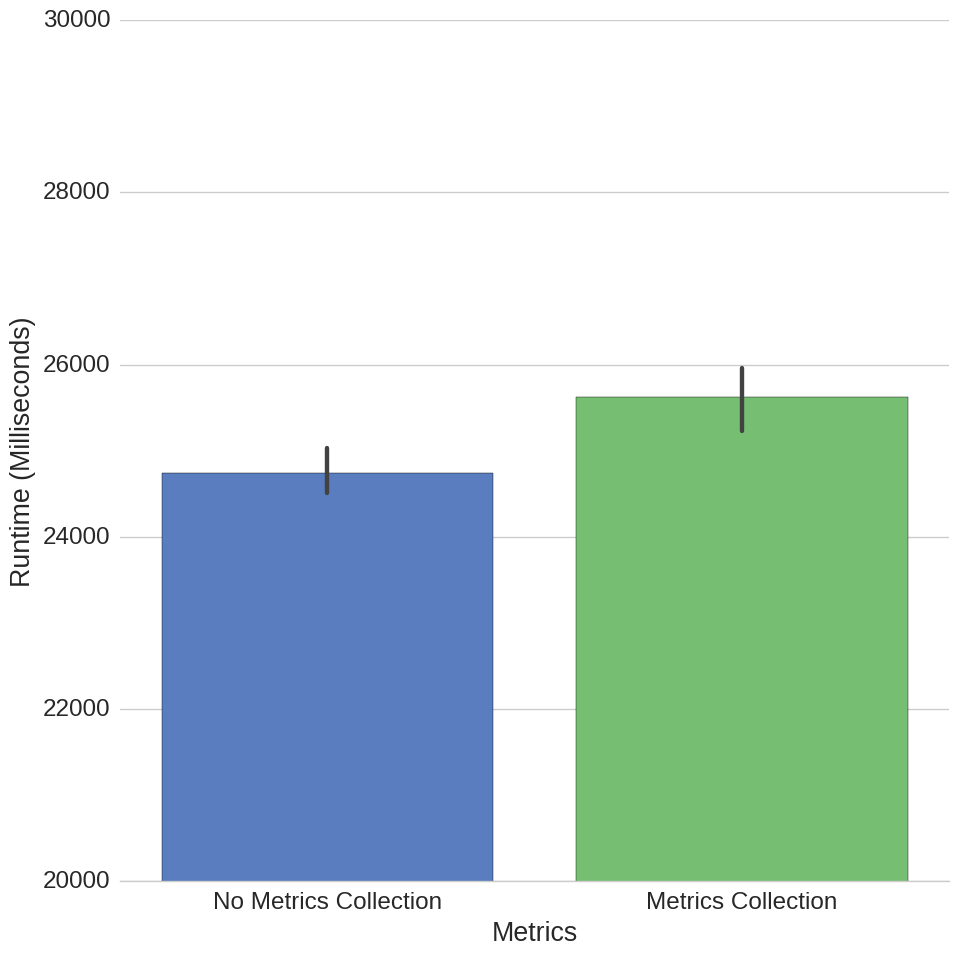
\includegraphics[width=\textwidth]{graphics/experiment1.png}
	\caption{Experiment 1 results}
	\label{fig:results_ex1}
\end{figure}

\begin{table}[H]
\centering
	\begin{tabular}{|c|c|}
		\hline
		Average delay added & 877ms \\
		\hline
		Percentage of total runtime & 3.5\% \\
		\hline
	\end{tabular}
	\caption{Experiment 1 Results Analysis}
	\label{table:results_experiment_1_results_analysis}
\end{table}

%% LaTeX2e file `ex_params/ex1_params.tex'
%% generated by the `filecontents' environment
%% from source `Report' on 2017/03/25.
%%
\begin{table}
\centering
 \begin{tabular}{|c|c|}
  \hline
  Number of tasks & 100,000 \\
  \hline
  Task Grain & 100,000 Repeats \\
  \hline
  Task Grain Distribution & Uniform \\
  \hline
  Number of CPU cores & 4 \\
  \hline
  Number of threads used & 4 \\
  \hline
  Thread pinning & Uniform \\
  \hline
  Schedule & Dynamic Chunks (Chunk Size = 1000) \\
  \hline
 \end{tabular}
\caption{Experiment 1 Parameters}
\iflabela
\label{table:evaluation_ex1_parameters}
\fi
\labelatrue
\end{table}




\subsection{Experiment 2 - Absolute Performance}

In this experiment, the total run times of three implementations are measured. One sequential implementation, a standard modern parallel implementation utilizing OpenMP, and our implementation of map\_array. Our implementation is running with no plasticity for the moment, and with no messaging functionality at all. This is so it is comparable to a standard parallel implementation, since the purpose of this experiment is to test our baseline performance.

Figure \ref{fig:results_ex2} shows us that with a single thread, our performance is similar to a sequential implementation, and as we increase the thread count, our performance scales accordingly. Overall, this shows that our implementation performs on a par with current parallel implementations, providing a good baseline performance. 



\begin{figure}
	\centering
	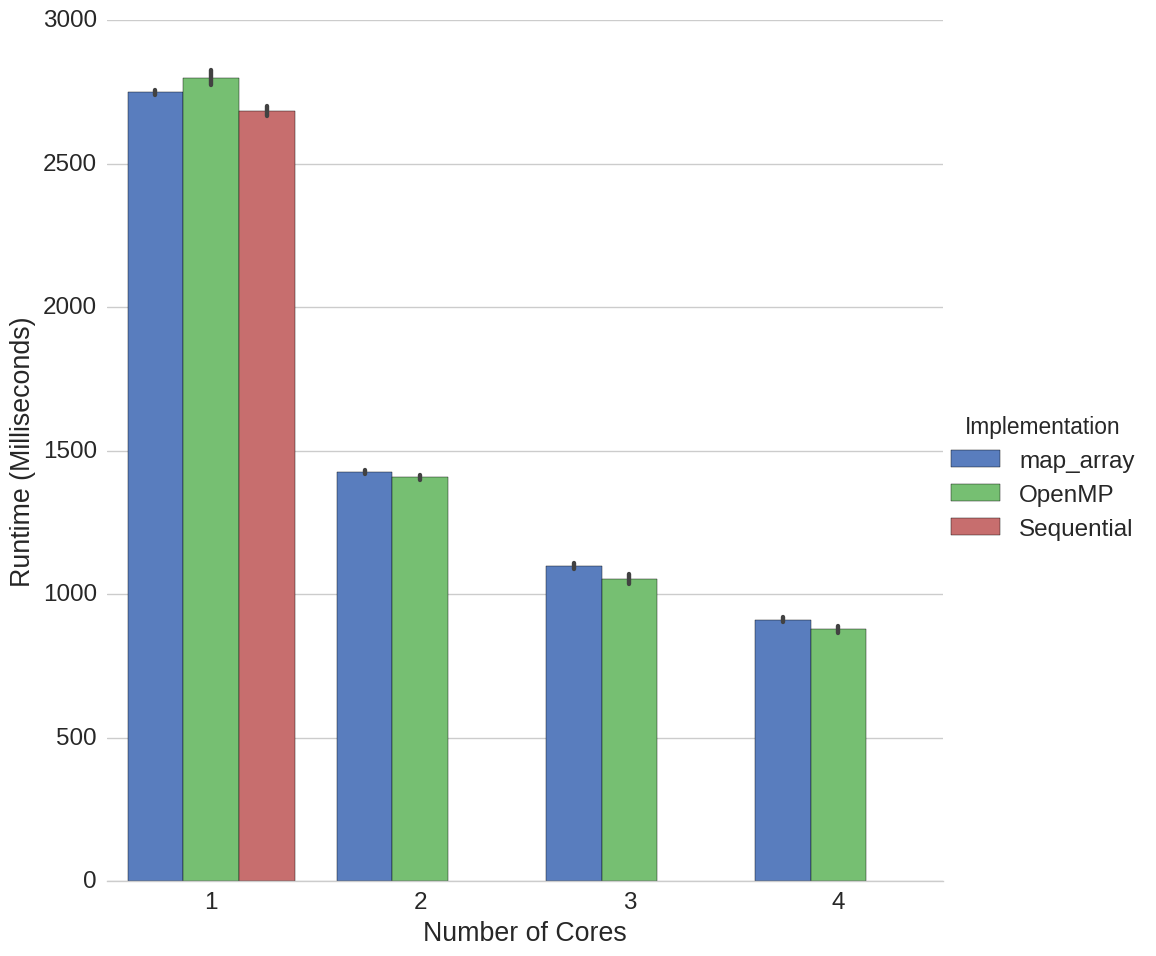
\includegraphics[width=\textwidth]{graphics/experiment2.png}
	\caption{Experiment 2 results}
	\label{fig:results_ex2}
\end{figure}

%% LaTeX2e file `ex_params/ex2_params.tex'
%% generated by the `filecontents' environment
%% from source `Report' on 2017/03/25.
%%
\begin{table}
\centering
 \begin{tabular}{|c|c|c|c|}
  \hline
  Number of tasks & 10,000 \\
  \hline
  Task Grain & 1,000,000 Repeats \\
  \hline
  Task Grain Distribution & Uniform \\
  \hline
  Number of CPU cores & 4 \\
  \hline
  Number of threads used & \specialcell{1, \\ 2, \\ 3, \\ 4} \\
  \hline
  Thread pinning & Uniform \\
  \hline
  Schedule & Static \\
  \hline
 \end{tabular}
\caption{Experiment 2 Parameters}
\iflabelb
\label{table:evaluation_ex2_parameters}
\fi
\labelbtrue
\end{table}




\subsection{Experiment 3 - Plasticity And Contention Aware Scheduling Framework Overhead}

This experiment was designed to assess the amount of overhead added by plasticity and the contention aware scheduling framework. The results are interesting, because we would expect the runtime to only increase with the added overhead, but we have two cases where the runtime decreases. 

With our smallest array size of 1000, we see an increase of 2ms, which is 2.7\% of the total runtime. These results are very close, and within the margin of error. 

Our other results both show a decrease in runtime, again both within the margin of error. Repeat experiments to reduce the variance would help, and running them on a VM may introduce more variance than in a non-virtualized system.

The overall conclusion from this experiment, is that the added overhead is negligible when measuring the total runtime, with a wide selection of array sizes.



\begin{figure}[H]
	\centering
	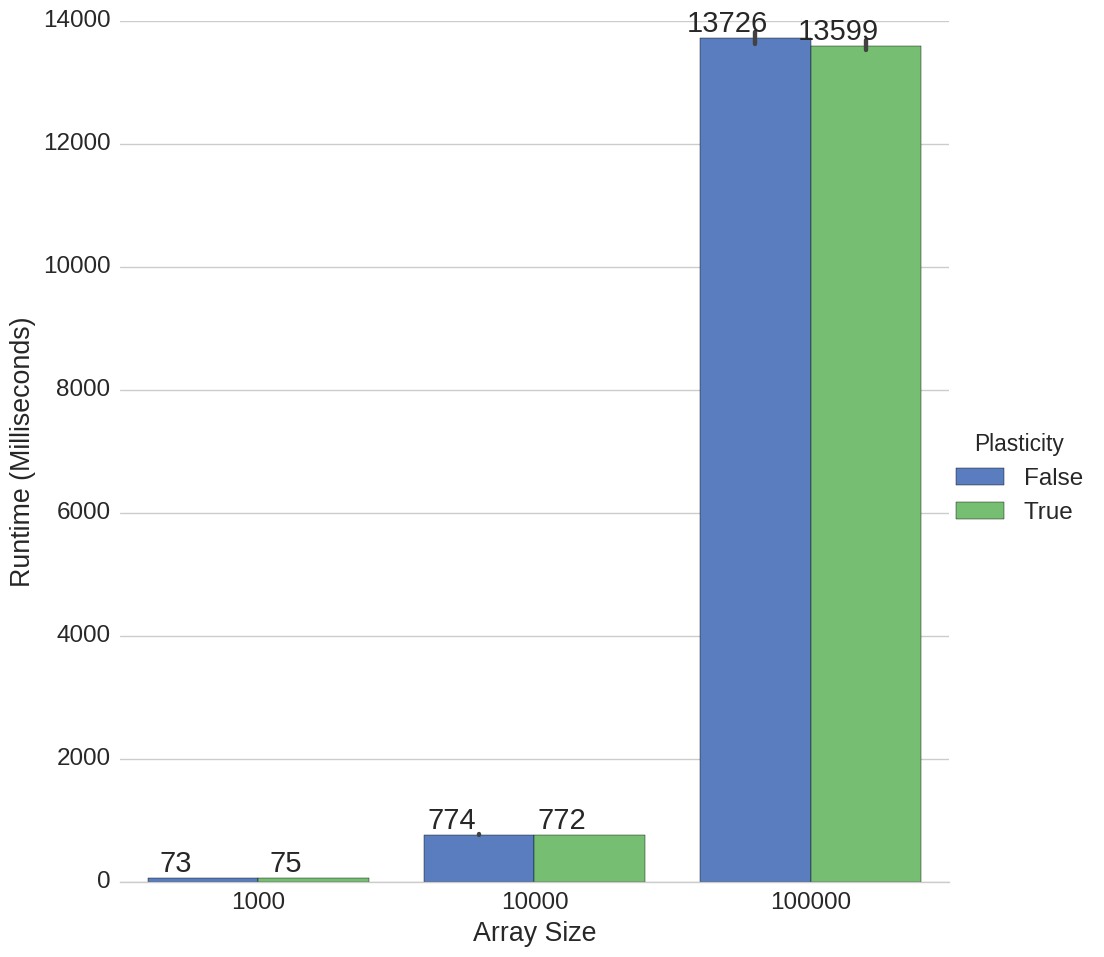
\includegraphics[width=\textwidth]{graphics/experiment3.png}
	\caption{Experiment 3 results}
	\label{fig:results_ex3}
\end{figure}

\begin{table}[H]
\centering
	\begin{tabular}{|c|c|}
		\hline
		Average delay added (Few tasks) & 2ms \\
		\hline
		Percentage of total runtime (Few tasks) & 2.7\% \\
		\hline
		\hline
		Average delay added (Med. tasks) & -2ms \\
		\hline
		Percentage of total runtime (Med tasks) & N/A \\
		\hline
		\hline
		Average delay added (Many tasks) & -127ms \\
		\hline
		Percentage of total runtime (Many tasks) & N/A \\
		\hline
	\end{tabular}
	\caption{Experiment 3 Results Analysis}
	\label{table:results_experiment_3_results_analysis}
\end{table}

%% LaTeX2e file `ex_params/ex3_params.tex'
%% generated by the `filecontents' environment
%% from source `Report' on 2017/03/25.
%%
\begin{table}
\centering
 \begin{tabular}{|c|c|}
  \hline
  Number of tasks & 100,000 10,000 1,000 \\
  \hline
  Task Grain & Medium \\
  \hline
  Task Grain Distribution & Uniform \\
  \hline
  Number of CPU cores & 4 \\
  \hline
  Number of threads used & 4 \\
  \hline
  Thread pinning & Uniform \\
  \hline
  Schedule & Dynamic Chunks \\
  \hline
 \end{tabular}
\caption{Experiment 3 Parameters}
\iflabelc
\label{table:evaluation_ex3_parameters}
\fi
\labelctrue
\end{table}




\subsection{Experiment 4 - Schedule Choice Importance}

This experiment was designed to highlight the importance of choosing the correct schedule, and how we can benefit from runtime plasticity. We have a biased set of tasks, (first quarter of which are large tasks, the rest small,) meaning the static schedule will perform poorly, and the dynamic schedules will fare well.

This is reflected in the results, where we see the dynamic schedules perform almost three times as well as the static schedule. Also included is a case where we start with the static schedule, and then switch to dynamic chunks after five seconds. We see it perform on a par with our dynamic schedules, again greatly improving upon the static schedule.

There is a small difference between our dynamic chunks and dynamic individual schedules. With a chunk size of 1,000, our dynamic individual schedule accesses the bag of tasks 1,000 times as often. Considering that it is implemented in shared memory, it makes sense that this penalty is not large. If retrieving tasks was more costly, it would affect the dynamic individual schedule proportionately more than the dynamic chunks schedule. We also have a variety of task sizes, meaning the time between bag accesses varies. In turn, this means threads are less likely to contend with each other when attempting to obtain the mutex to access the bag.

In our plastic schedule, we change from static to dynamic\_chunks after 5 seconds. In these first 5 seconds, all threads will still have tasks to process, meaning we still have maximum throughput. Since we change to a dynamic schedule before we have any down time, we match the performance of a constant dynamic schedule.



\begin{figure}
	\centering
	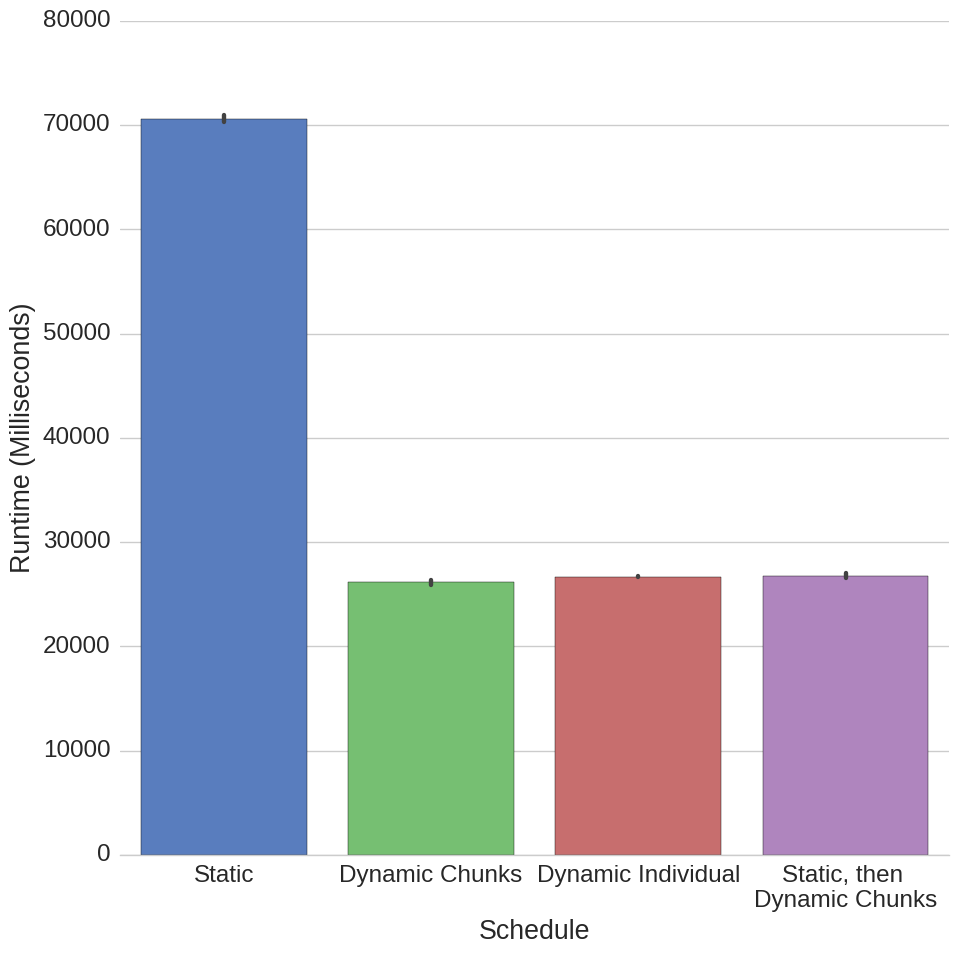
\includegraphics[width=\textwidth]{graphics/experiment4.png}
	\caption{Experiment 4 results}
	\label{fig:results_ex4}
\end{figure}

%% LaTeX2e file `ex_params/ex4_params.tex'
%% generated by the `filecontents' environment
%% from source `Report' on 2017/03/25.
%%
\begin{table}
\centering
 \begin{tabular}{|c|c|}
  \hline
  Number of tasks & 100,000 \\
  \hline
  Task Grain & Large and small \\
  \hline
  Task Grain Distribution & Biased \\
  \hline
  Number of CPU cores & 4 \\
  \hline
  Number of threads used & 4 \\
  \hline
  Thread pinning & Uniform \\
  \hline
  Schedule & \specialcell{Static, \\ Dynamic Chunks (Chunk Size = 1,000), \\ Dynamic Chunks (Chunk Size = 1) \\ Static, then dynamic chunks after 5 seconds} \\
  \hline
 \end{tabular}
\caption{Experiment 4 Parameters}
\iflabeld
\label{table:evaluation_ex4_parameters}
\fi
\labeldtrue
\end{table}




\subsection{Experiment 5 - Absolute Multiprogramming Performance}

The purpose of this experiment is to investigate the absolute performance of our library in a situation with multiple applications. We compare two situations, the first, named anarchy, is where both programs are run with four threads with no plasticity or contention aware scheduling. This is a typical situation for a multiprogramming system. In the second situation, we use plasticity and contention aware scheduling, where we start with four threads in program 1, once program 2 starts we reduce this to two, and assign two threads to program 2. Once program 2 is finished, we switch back to using four threads in program 1.

For a further investigation into the performance of our library, and on a hunch, we also ran the experiment with different message checking intervals. This means that each program's main thread sleeps for Nms in between checks for whether the computation is complete or if it has any messages.

Looking at the results, our library is consistently faster than anarchy, which is a promising sign. We also significantly reduce the variance using our library, possibly due to the reduced thread switching. Comparing the different sleep times, we see that significant improvements can be made, if we tune this variable correctly. Since we are reducing some overhead by making this interval longer, (with the compromise of a slower reaction speed to messages), we could reason that if the library were more sophisticated, and if we thoroughly optimized our code, we may see substantial performance gains.

There is an interesting performance gain going from a 20ms checking interval to a 100ms interval. While unusual, it held for the 50 repeats, so it is not an isolated case. Due to time constraints, this could not be investigated further, but this could be a possibility for the future work in the next year of this MInf project.



\begin{figure}
	\centering
	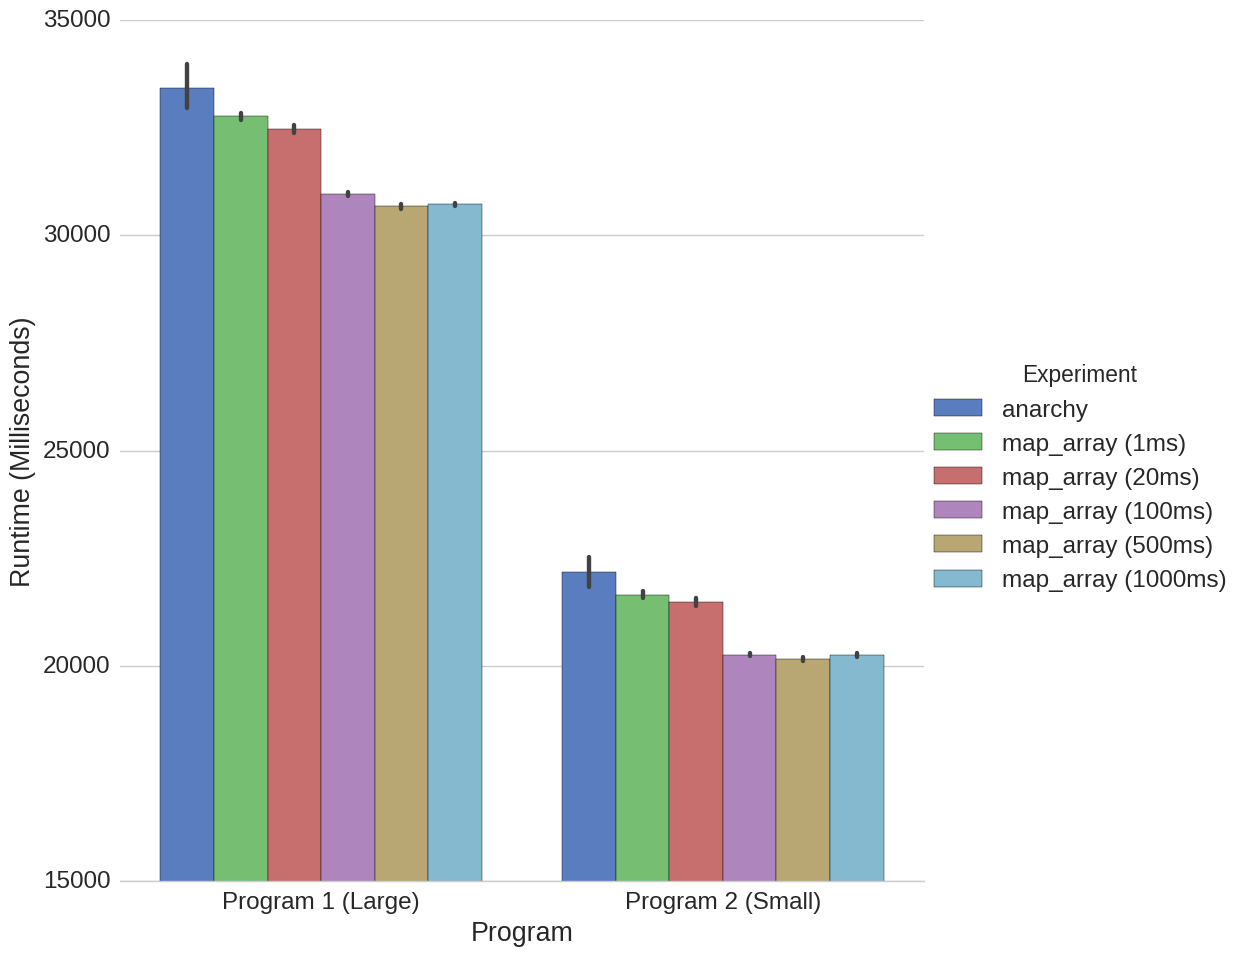
\includegraphics[width=\textwidth]{graphics/experiment5.png}
	\caption{Experiment 5 results}
	\label{fig:results_ex5}
\end{figure}

%% LaTeX2e file `ex_params/ex5_params.tex'
%% generated by the `filecontents' environment
%% from source `Report' on 2017/03/25.
%%
\begin{table}
\centering
 \begin{tabular}{|c|c|}
  \hline
  Program 1 & \\
  \hline
  Number of tasks & 30,000 \\
  \hline
  Task Grain & 10,000,000 Repeats \\
  \hline
  Task Grain Distribution & Uniform \\
  \hline
  Number of CPU cores & 4 \\
  \hline
  Number of threads used & \specialcell{4 \\ 4, then 2, then 4} \\
  \hline
  Thread pinning & \specialcell{Loose, \\ Uniform} \\
  \hline
  Schedule & Dynamic\_individual \\
  \hline
 \end{tabular}

 \begin{tabular}{|c|c|}
  \hline
  Program 2 & \\
  \hline
  Number of tasks & 15,000 \\
  \hline
  Task Grain & 10,000,000 Repeats \\
  \hline
  Task Grain Distribution & Uniform \\
  \hline
  Number of CPU cores & 4 \\
  \hline
  Number of threads used & \specialcell{4 \\ 2} \\
  \hline
  Thread pinning & \specialcell{Loose, \\ Uniform} \\
  \hline
  Schedule & Dynamic\_individual \\
  \hline
 \end{tabular}
\caption{Experiment 5 Parameters}
\iflabele
\label{table:evaluation_ex5_parameters}
\fi
\labeletrue
\end{table}




\section{Conclusion}

In this section, we discuss the implications of each experiment, and what they mean for the future of the project. 

Experiment 1 investigates the overhead added by detailed metrics collection. These metrics were mostly used during development, and as such were disabled for future experiments to minimize their performance impact. 

Experiment 2 establishes a baseline of performance, confirming that we are on a par with current parallel programming approaches. This is a positive result, and confirms that our approach does not concede significant overhead. 

Experiment 3 investigates the overhead involved in contention aware scheduling and plasticity. The results build upon the conclusion of experiment 2, in that we do not add any significant overhead, this time by measuring the overhead of plasticity and contention aware scheduling.

Experiment 4 is a demonstration of the value of choosing the correct schedule, and shows the benefits of plasticity. 

Experiment 5 confirms that we can improve upon our standard implementation with plasticity and contention aware scheduling. We also see reduced variability, both of which are promising results for the early stages of this project. It provides a solid foundation for the next phase in the following year. We also show that we can improve our performance further by optimizing and tuning the code, again providing promising work for the future.

A future system would be useful in any performance orientated application, even when the machine will only be running a single instance, as we can still optimize the implementation to the environment on that machine (as demonstrated in experiment 4.) It would, however, come into its own when we have multiple instances running simultaneously on a machine, a common situation with modern multiprogramming machines.

Overall, the first year of this project has provided a solid foundation for the work to be done next year, and future work for others following the completion of the project.

\chapter{Future Work And Conclusions}
\label{chapter:future_work_and_conclusions}
%!TEX root = ../Report.tex

This chapter discusses further work that could be done to advance this project, and a personal reflection upon the project as a whole. There is a large scope for development here, and as such, we will select a subset of tasks to focus on in the second year. We also discuss possibilities for future applications, and the library's utility beyond simply investigating the nature of the problem.



\section{Future Development}

Here we provide an overview for possible work to be done in the future. We split the tasks into work for the second phase of this MInf project, and interesting work for successors:

Next year:

\begin{itemize}
	\item Improved experiment framework, with support for experiments involving multiple programs
	\item Experiment with different array access patterns, and investigate how they affect performance
	\item Experiment with different types of task, such as different bottlenecks (CPU bottleneck/Memory bottleneck) 
	\item Test the library on a variety of hardware and systems
	\item Make work interruptable, currently, once we have assigned tasks, a worker thread cannot be interrupted. This means that the static schedule, which assigns all tasks at once, cannot be interrupted/switched without manually forcing it to do so
	\item Currently, we only have the map array pattern. More patterns could be implemented, as a real-world version of our library would provide multiple common patterns of parallel programming, and may even utilize multiple backends allowing for different features (e.g. Standard Pthreads, OpenCL/CUDA for multi-GPU computation).
	\item Support for different parallel programming backends, possibly utilizing more exotic hardware such as GPUs 
	\item Implementing some algorithm for automatic parameter tuning. It's feasible that the system could assess both the tasks presented and the environment (e.g. the particulars of the machine, currently running applications), and automatically allocate the resources of the machine so we perform in the most efficient manner.
	\item Moving away from the virtual machine for experimentation. The VM may introduce variance into our experiments, an limits us to the experiments we can perform. For example, we saw unusually large runtimes with large input arrays. this is because the array was larger than the memory assigned to the VM, meaning it was not entirely kept within memory.
\end{itemize}

Follow on work:

\begin{itemize}
	\item Different methods of task distribution could be investigated, such as a distributed bag of tasks or adding task stealing
	\item The project could be adapted for use in a distributed system, where we may have a variety of hardware, machines, and tasks to contend with. In this scenario, we would have a large amount of input parameters to our scheduler, resulting in a complex problem. We may have programs spread across multiple machines, we need to consider what machine is best to run a particular program on, and what other programs are running on that machine. The system could feasibly be controlled by a single controller application, serving requests from each machine, or it could be distributed across the machines, or we may use a hierarchy, with a controller per machine and a master controller. 
	\item We currently optimize our library for performance, however the system may also be useful in non-performance orientated applications, for example, we may want to optimize energy usage for mobile applications. We could also optimize for a mix of performance and energy, which, with studies reporting that \textit{the total cost of a server will be primarily a function of the power it consumes} \cite{datacentres}, would be useful in server farms or data centres.
	\item In deciding what resources to allocate to which program, we could implement a priority system. Both an internal priority system and a user controlled priority system would be useful. In an internal priority system, we would asses attributes of each program, and possibly assign more resources to one than the other (e.g. if one program scales better than another, we may decide to grant it extra CPU cores until it is complete.) A user controlled priority system would deal with cases where some programs are more or less important compared to other programs to the user. We could allow the user to manually control priorities, or possibly even the distribution of resources. 
\end{itemize}



\subsection{Personal Reflection}

In this section we provide a personal reflection on the first year of this project, and thoughts for the future.

Working on this project, I have learned much about parallel programming, C++ programming, and managing a large software engineering project. I had not done any of these things prior to this project. Overall I am pleased with the results of the project so far. I've completed,and indeed exceeded, all the goals I set at the start of the year.

Looking back, it is apparent that the project would have benefited from simultaneous development of the report, and the development of more sophisticated testing software. Whilst the current system could be adapted to the requirements of the experiments, this would have made it easier to perform experiments. This will therefore definitely be an improvement undertaken in the next year of this MInf project.

The outcome of this report has provided exciting results for next year, and I'm looking forward to implementing new features, and particularly to further experiments investigating the system. I would also like to again learn new things, particularly programming for GPUs, and more advanced inter-process communication. Hopefully, the project can be further improved, and leave an easy to extend code base for future students.

\newpage

\bibliographystyle{acm}
\bibliography{references} 

\end{singlespacing}

\end{document}